% ---------------------------------------------------------------------- %

\documentclass[letterpaper,10pt]{article}



\pagestyle{empty}

\usepackage[table]{xcolor}
\usepackage{color, colortbl}
\usepackage{tabularx}
\usepackage{amssymb}
\usepackage{enumerate}

\definecolor{LightGray}{gray}{0.9}

\usepackage{amsmath}
\usepackage{amscd}
\usepackage{url}

\usepackage{graphicx}


\title{Picking Travel Times}
\author{Northwestern Seismology Group}
\date{\today}

\begin{document}
\maketitle

% ************************************************************* %
%                                                               %
%                       PICK TRAVEL TIMES                       %
%                                                               %
% ************************************************************* %

\section{Picking travel times}

% ----------------------------------------------- %

\subsection{Getting into the right directory}

In the terminal, cd into the directory with all the pkl files you want to run. You want to run either the \verb".bht" or \verb".bhz" files. \texttt{bht} files are for $S$-waves and \texttt{bhz} files are for $P$-waves. PKL is a bundle of SAC files. Each SAC file is a seismogram, but since you there may be many seismograms from various stations for each event, we bundle them into a PKL file so we only have to import one file into AIMBAT, not a few hundred of them.

% ----------------------------------------------- %

\subsection{Running \texttt{ttpick.py}}

\begin{verbatim}
	ttpick.py ___.bhz.pkl
\end{verbatim}

A GUI should pop up if you successfully ran it.  

\begin{figure}[h!]
  \centering
  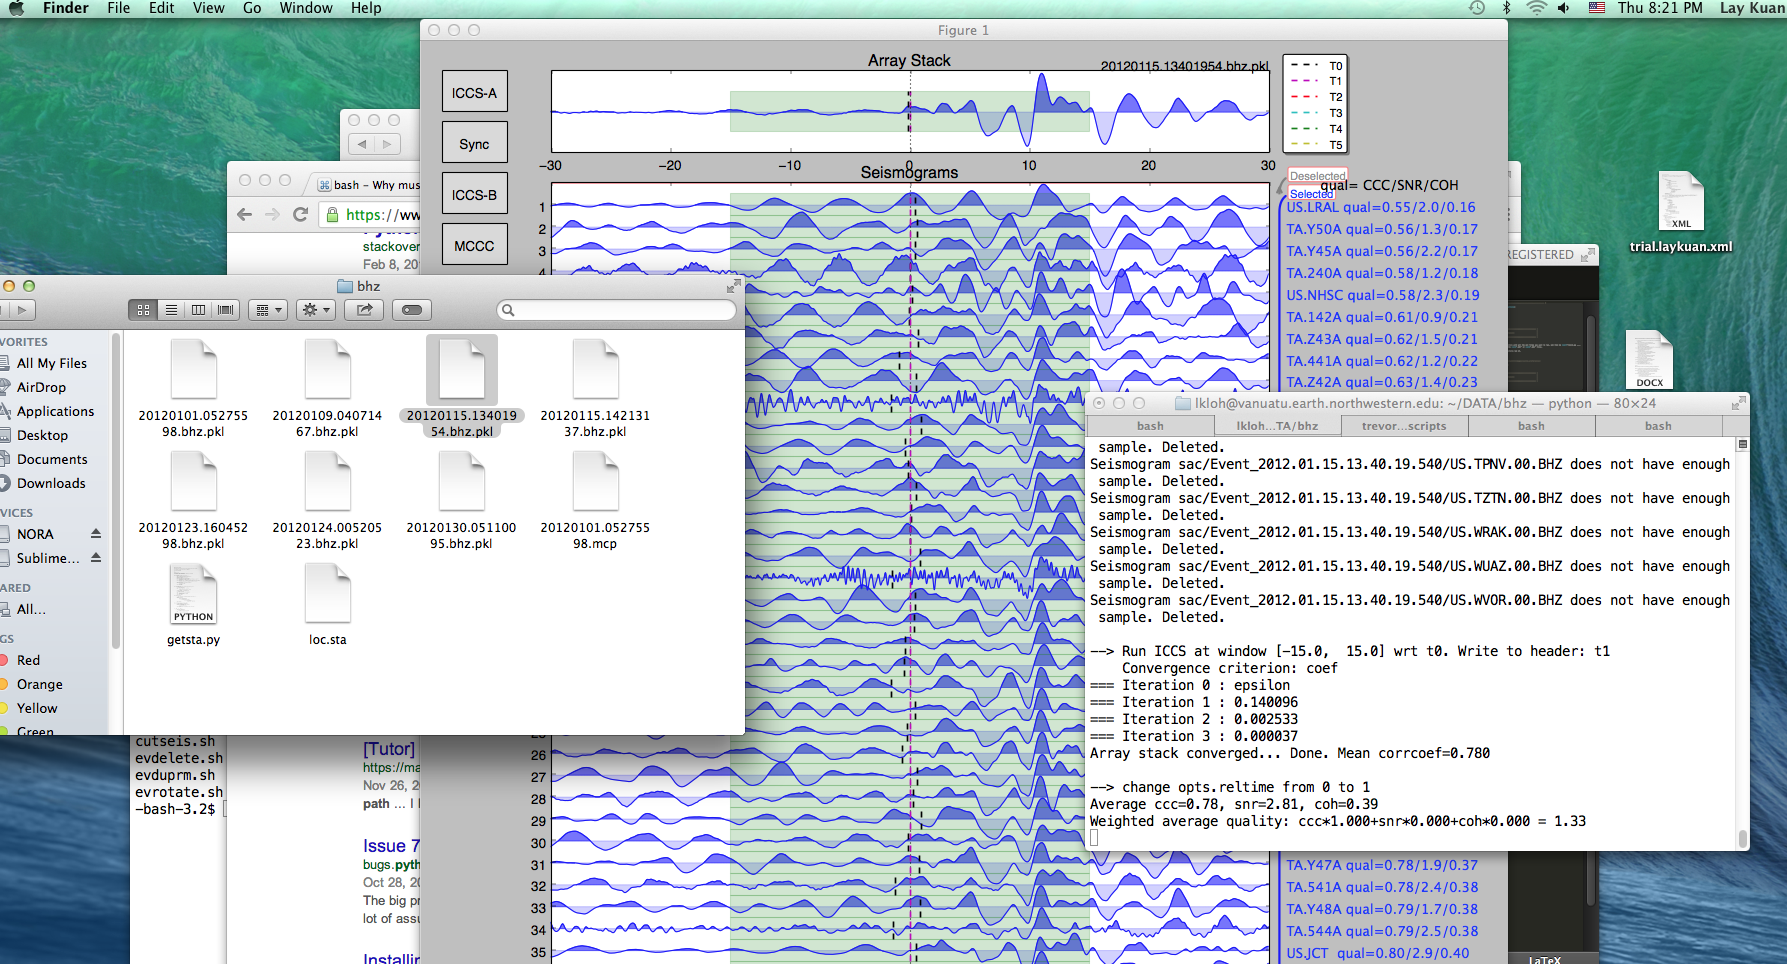
\includegraphics[width=0.5\textwidth]{images/pick_travel_times}
  \caption{Pick travel times}
  \label{fig:pick_travel_times}
\end{figure}

Note that if you click on the buttons, they will not work until you move the mouse off them.

% ----------------------------------------------- %

\subsection{Get rid of really bad seismograms}

If there are any really bad seismograms, you can click on them to deselect them. 

Remember to save your work periodically once you start picking your travel times, otherwise if AIMBAT crashes, you lose it. 

% ----------------------------------------------- %

\subsection{ICCC-B}

Hit the \framebox[1.1\width]{ICCC-B} button to begin the initial cross-correlations. These appear as red lines. 

We are not using \framebox[1.1\width]{ICCC-A} here, but these are the theoretical arrival times, marked in black. 

% ----------------------------------------------- %

\subsection{Manually pick the arrival times using \texttt{t2}}

For an earthquake, it is expected that the arrival times should be identical in an idealize situation. However, since stations are located in 3D space, this is not necessarily the case. Fror earthquakes of magnitude 7.0 and above, usually yhe arrival times are very well aligned as the signal is high.

We manually pick the the arrival times to align them. Click on the GUI window, hover over the correct spot where you want to pick the new travel time, and type \texttt{t2}. A red line should appear exactly where your mouse was. 

Also pick the arrival time on the array stack. 

% ----------------------------------------------- %

\subsection{MCCC}

Hit \framebox[1.1\width]{MCCC} to run the Multi-Channel cross-correlation. Do not high \framebox[1.1\width]{ICCC-A} or \framebox[1.1\width]{ICCC-B} again, or all your work will be erased. 

% ----------------------------------------------- %

\subsection{SACP2 to check for outlier seismograms}

Hit \framebox[1.1\width]{SACP2} and go to the last figure, (D). Zoom in to have a better look. Zooming in doesn't always work well; close and reopen the SACP2 window if there are problems. 

Click on the outliers that stray from the main group of stacked seismograms. The terminal will output the names of the seismograms that you clicked on, so you can return to the main GUI window and readjust the travel times.

\begin{figure}[h!]
  \centering
  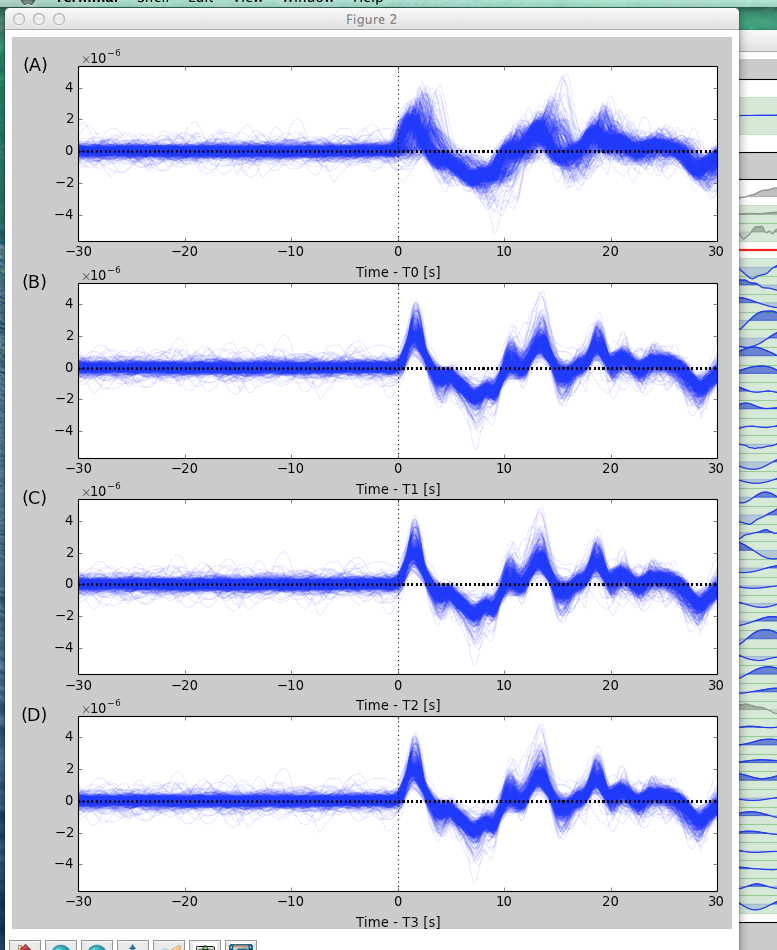
\includegraphics[width=0.5\textwidth]{images/SACP2_popup}
  \caption{SACP2 popup}
  \label{fig:SACP2_popup}
\end{figure}

% ----------------------------------------------- %

\subsection{Go through the badly aligned seismograms and realign the travel times manually}

By default, the worst seismograms are on the first page, and as you click through the pages, the quality of the seismograms gradually gets better. Keep using \texttt{t2} to realign the arrival times so that the peaks of all the seismograms are nicely aligned. Remember to zoom in to have a better look.

However, you may which to sort the seismograms in alphabetical order so that you can find the bad seismogrrams and correct them more easily. Run 

\begin{verbatim}
	ttpick.py -s -i ___.bhz.pkl
\end{verbatim}

and scroll through the pages. Notice that clicking through the pages may be slow, move the mouse around and off/on the GUI window to stop it stalling. You can also hit MCCC to jump back to the front page. 

The seismograms are stretched to fit together, but they may be scaled differently. 

% ----------------------------------------------- %

\subsection{What the alignments stand for}

TO: Theoretical Arrival

T1: Pick from initial cross correlation

T2: Travel Time pick

T3: MCCC pick

T4: Zoom in

% ************************************************************* %
%                                                               %
%                       PICK TRAVEL TIMES                       %
%                                                               %
% ************************************************************* %

\section{Post Processing}

\subsection{Getting the output}

In the same folder as the initial PKL file you ran \texttt{ttpick.py} on, you can find the output list with extension \texttt{<event name>.mcp}, which contains the travel time arrivals. 

\begin{figure}[h!]
  \centering
  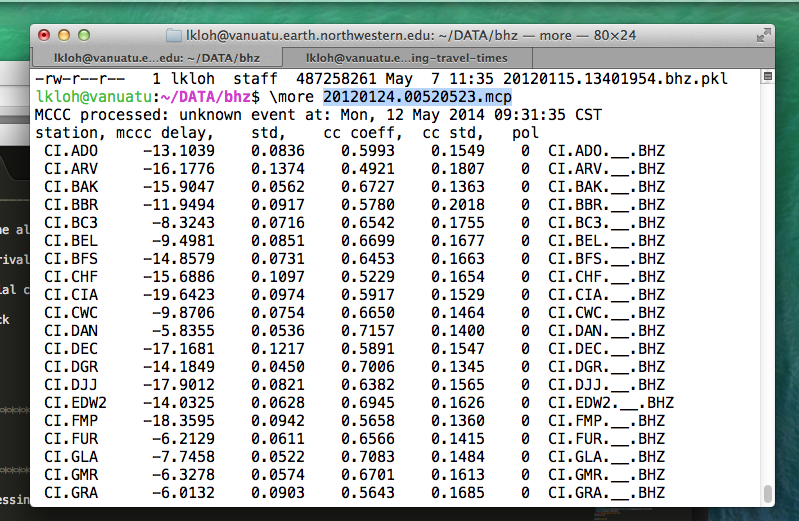
\includegraphics[width=0.5\textwidth]{images/output_list}
  \caption{Output list}
  \label{fig:output_list}
\end{figure}

\subsection{Getting the stations of the seismograms chosen}

Run \verb"getsta.py" in the additional scripts (not on Github for now). It gives the unique list of stations where the seismograms came from. You need to run it with the list of all \verb"pkl" files chosen after you saved to. You so this \verb"./getsta.py *.pkl". 

\begin{figure}[h!]
  \centering
  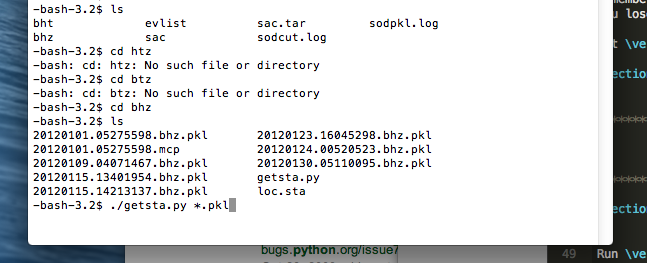
\includegraphics[width=0.5\textwidth]{images/count_stations}
  \caption{count stations}
  \label{fig:count_stations}
\end{figure}

\end{document}

% --------------------------------- END --------------------------------- %
